\section{Palindromos-Gram\'atica libre de contexto}
\subsection{ Descripci\'on del programa}
\justify
El siguiente programa genera palindromos de cadenas binarias, esto se logra gracias a las siguientes reglas de produccion de la gramatica:\\
\begin{center}
1.-S--$>$e\\
2.-S--$>$0\\
3.-S--$>$1\\
4.-S--$>$0S0\\
5.-S--$>$1S1\\
\end{center}
El programa cuenta con un modo manual y autom\'atico, con el cual se podr\'a elegir el tama\~no del palindromo, como salidas se obtendr\'a en un archivo la forma en que se fue generando y en otro archivo la regla que se utilizo en cada caso.
\\
\subsection{C\'odigo}
El c\'digo utilizado para la resoluci\'on del problema se muestra a continuaci\'on:\\

C\'odigo:palindromo.py

\lstset{language=Python, breaklines=true, basicstyle=\footnotesize}
\begin{lstlisting}[frame=single]
	import random;

def IniciarArchivo():
	archivo=open("palindromo.txt","w")
	archivo.close
	historia=open("historiaPal.txt","w")
	historia.close

def Run(pal,longitud,par):
	try:
		archivo=open("palindromo.txt","a")
		historia=open("historiaPal.txt","a")
	except:
		exit()
	archivo.write("S")
	exito=generar_palindromo1(archivo,pal,longitud,par,historia)
	archivo.write("\n\n")
	historia.write("------\n\n")
	archivo.close
	historia.close
	return exito

def opcion_fin(par):
	if(par==True):
		op=1
	else:
		op=random.randint(2,3)
	return op

def opcion_inicio():
	op=random.randint(4,5)
	return op

def regla1(pal,historia):
	pal=pal.replace("S","")
	historia.write("\n1.-S-->e")
	return pal

def regla2(pal,historia):
	pal=pal.replace("S",'0')
	historia.write("\n2.-S-->0")
	return pal

def regla3(pal,historia):
	pal=pal.replace("S",'1')
	historia.write("\n3.-S-->1")
	return pal

def regla4(pal,historia):
	pal=pal.replace("S","0S0")
	historia.write("\n4.-S-->0S0")
	return pal
def regla5(pal,historia):
	pal=pal.replace("S","1S1")
	historia.write("\n5.-S-->1S1")
	return pal

def generar_palindromo1(archivo,pal,longitud,par,historia):
	
	if(longitud>1):
		
		opcion=opcion_inicio()
		if(opcion==4):
			pal=regla4(pal,historia)
			archivo.write("\n"+pal)
		if(opcion==5):
			pal=regla5(pal,historia)
			archivo.write("\n"+pal)

	if(longitud==1):
		opcion=opcion_fin(par)
		if(opcion==1):
			pal=regla1(pal,historia)
			archivo.write("\n"+pal)
		if(opcion==2):
			pal=regla2(pal,historia)
			archivo.write("\n"+pal)
		if(opcion==3):
			pal=regla3(pal,historia)
			archivo.write("\n"+pal)
	if (longitud==0):
		return 1
	longitud=longitud-1
	pal=generar_palindromo1(archivo,pal,longitud,par,historia)

\end{lstlisting}
\vspace{1.5cm}
C\'odigo:main.py

\lstset{language=Python, breaklines=true, basicstyle=\footnotesize}
\begin{lstlisting}[frame=single]
import palindromo
import random

def longitud():
	x=random.randint(0,1000);
	return x

palindromo.IniciarArchivo()
def menu():
	print("-----Menu-----")
	print("1.-Modo Manual")
	print("2.-Modo Automatico")
	print("3.-Salir")

while True:
	menu()
	opcion=input("Seleccione una opcion: ")
	if(opcion=="1"):
		tamanio=input("Ingrese un tamanio de cadena: ")
		print(tamanio)
		tamanio=int(tamanio)
		if(tamanio%2==0):
			g=palindromo.Run("S",(tamanio/2)+1,True)
		else:
			tamanio=int(tamanio/2)+1
			g=palindromo.Run("S",tamanio,False)

		while True:
			try:
				seln=input("Desea regresar al menu\n1.-Si\n2.-No\n- ")
				seln=int(seln)
			except:
				exit()

			if(seln==1):
				break
			elif(seln==2):
				exit()
			else:
				continue
	elif(opcion=="2"):
		tamanio=longitud()
		print(tamanio)
		if(tamanio%2==0):
			g=palindromo.Run("S",(tamanio/2)+1,True)
		else:
			tamanio=int(tamanio/2)+1
			g=palindromo.Run("S",tamanio,False)

		while True:
			try:
				seln=input("Desea regresar al menu\n1.-Si\n2.-No\n- ")
				seln=int(seln)
			except:
				exit()

			if(seln==1):
				break
			elif(seln==2):
				exit()
			else:
				continue

	elif(opcion=="3"):
		exit()

	else:
		print("Seleccione una opcion correcta")

\end{lstlisting}
\newpage

\subsection{Pruebas}
A continuaci\'on se mostraran algunas im\'agenes capturadas al momento de ejecutar el programa, dichas im\'agenes mostraran los resultados obtenidos.\\
\vspace{1.0cm}
Para el modo manual:\\
\begin{figure}[H]
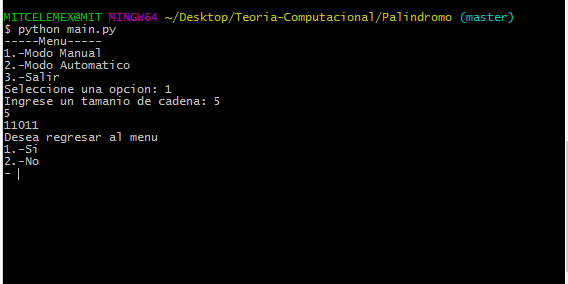
\includegraphics[width=\textwidth, height=7cm]{ModoManualPal.png}
\label{fig:manual_webay}
\caption{El tama\~no de la cadena sera de 5}
\end{figure}

\begin{figure}[H]
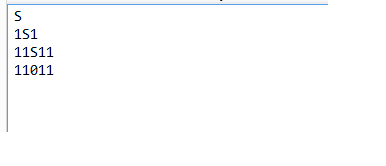
\includegraphics[width=\textwidth, height=7cm]{ArchivoPal.png}
\label{fig:manualtexto_alfabeto}
\caption{Evaluaci\'on de la gram\'atica}
\end{figure}

\begin{figure}[H]
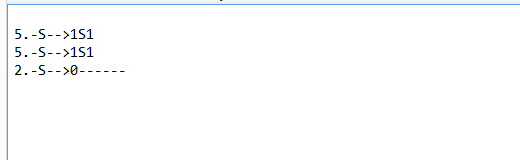
\includegraphics[width=\textwidth, height=7cm]{HistoriaPal.png}
\label{fig:manualtexto_alfabeto}
\caption{Historia de la evaluaci\'on de la gram\'atica}
\end{figure}

Para el modo autom\'atico:\\
\begin{figure}[H]
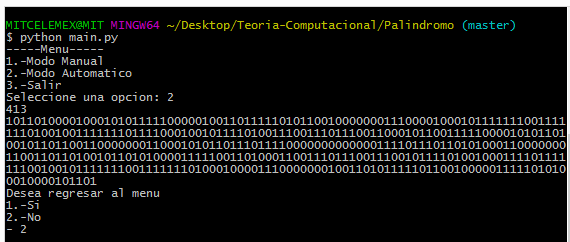
\includegraphics[width=\textwidth, height=7cm]{ModoAutomaticoPal.png}
\label{fig:auto_alfabeto}
\caption{Tama\~no generado autom\'aticamente}
\end{figure}

\begin{figure}[H]
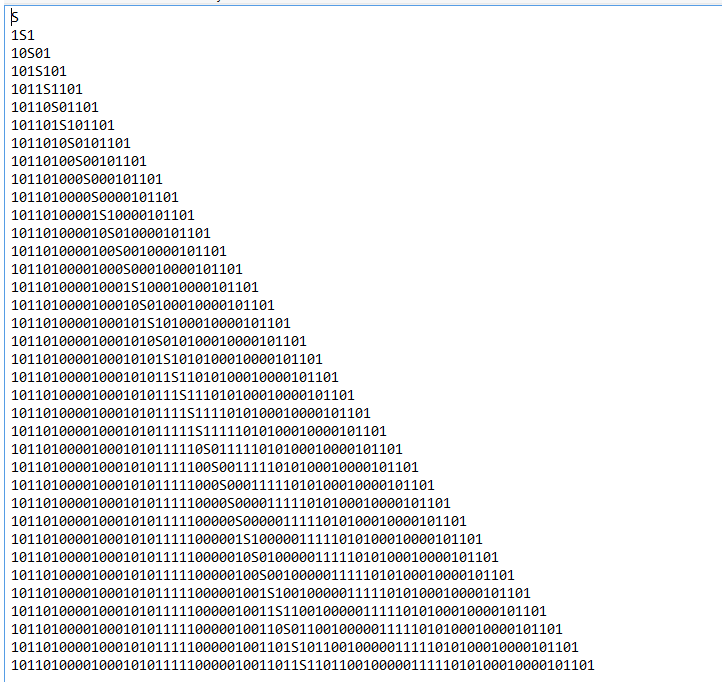
\includegraphics[width=\textwidth, height=7cm]{ArchivoHistoriaPal.png}
\label{fig:autotexto_alfabeto}
\caption{Historia de la evaluaci\'on del modo autom\'atico}
\end{figure}

\begin{figure}[H]
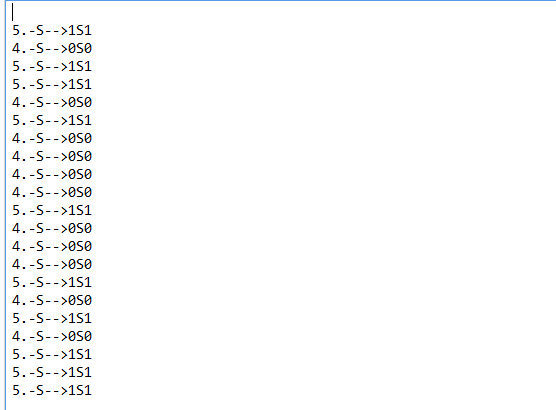
\includegraphics[width=\textwidth, height=7cm]{HistoriaPalA.png}
\label{fig:manualtexto_alfabeto}
\caption{Historia de la evaluaci\'on de la gram\'atica}
\end{figure}

\newpage